\section{Aquisição de Dados}
O circuito de aquisição de sinais sEMG é projetado para amplificar e filtrar o sinal captado pelos eletrodos antes de sua digitalização. O amplificador de instrumentação, como o INA128 ou o AD8221, é responsável pela amplificação diferencial do sinal com alta rejeição ao modo comum (CMRR), fundamental para eliminar interferências eletromagnéticas presentes no ambiente clínico e laboratorial.

Após a amplificação, o sinal passa por uma cadeia de filtros analógicos: um filtro passa-altas de segunda ordem (tipicamente Butterworth) com frequência de corte de 20 Hz remove componentes DC e artefatos de baixa frequência; um filtro passa-baixas com corte em 500 Hz limita a banda de interesse; e um filtro notch em 60Hz (padrão brasileiro) atenuar a interferência da rede elétrica. O sinal condicionado é então amostrado pelo conversor analógico-digital (ADC) do microcontrolador com frequência de amostragem de pelo menos 1 kHz (conforme o critério de Nyquist para a faixa de interesse).

\begin{figure}[htbp]
    \centering
    \caption{Fluxograma das etapas de amplificação e filtragem do sinal sEMG}    
    \label{fig:fluxogramafiltros}
    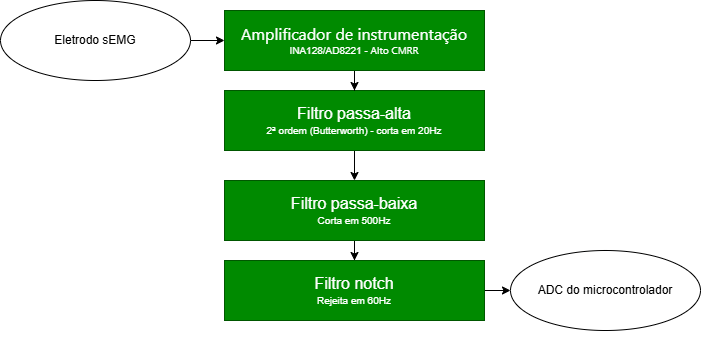
\includegraphics[width=0.8\textwidth]{2_fundamento_teorico/assets/FluxogramaFiltros.png}
    \fonte{Elaborado pelo autor (2026)}
\end{figure}